\documentclass[11pt]{article}

\usepackage[utf8]{inputenc}
\usepackage[T1]{fontenc}
\usepackage{amsmath,amssymb}
\usepackage{graphicx}
\usepackage{booktabs}
\usepackage{url}
\usepackage{hyperref}
\usepackage{xcolor}
\usepackage{listings}
\usepackage{float}
\usepackage{caption}
\usepackage[margin=1in]{geometry}
\usepackage{enumitem}
\usepackage{needspace}
\usepackage{tikz}
\usetikzlibrary{positioning,arrows.meta,shapes.geometric,fit,calc}

\hypersetup{
  colorlinks=true,
  linkcolor=blue!60!black,
  citecolor=blue!60!black,
  urlcolor=blue!60!black,
}

\lstset{
  basicstyle=\ttfamily\small,
  breaklines=true,
  frame=single,
  xleftmargin=1.5em,
  framexleftmargin=1em,
  backgroundcolor=\color{gray!5},
  aboveskip=1em,
  belowskip=1em,
}

\title{\textbf{From Fragile Glue to Governed Cognition}\\[0.5em]
{\large A Controlled Study of Blackboard Kernels for Modular AI Systems}}

\author{Emil Uzelac}

\date{February 2026}

\begin{document}

\maketitle

\begin{abstract}
As AI systems transition from isolated language models to autonomous and semi-autonomous agents, dominant failure modes shift from reasoning errors to orchestration failures. Modern agent architectures coordinate reasoning, tools, memory, and action through untyped text or loosely structured interfaces, resulting in unsupported beliefs, unsafe actions, and opaque failure cascades.

This study introduces the \textbf{Blackboard Kernel (BK)}, a governed cognitive substrate that enforces typed internal state, evidence-based belief commitment, and constraint-gated action execution. We formalize a threat model centered on orchestration-level failure, enumerate failure modes in hybrid agent systems, define architectural requirements for governed cognition, and demonstrate BK through concrete execution semantics, baseline failure walkthroughs, and controlled evaluation on Stripe payment refund tasks. We further validate BK with live LLM planners (GPT-OSS-20B, Qwen3-80B) to demonstrate that governance holds when the planning component is a language model rather than deterministic logic.

In a controlled evaluation of 1,200 episodes (6 Stripe refund tasks, 50 seeds, 4 agents), the deterministic BK agent achieves 100.0\% task success with zero unsafe actions, and the LLM-backed BK agent achieves 99.0\% task success with zero unsafe actions---while baseline architectures produce unsafe actions in 38.7--43.0\% of episodes. A separate domain-agnostic demonstration (temperature monitoring with adaptive constraint learning) confirms that the kernel's governance mechanisms generalize beyond the evaluation domain. These findings indicate that architectural governance, not model scale or planner implementation, is the primary bottleneck for trustworthy modular AI.

\medskip
\noindent\textbf{Keywords:} agent governance, blackboard architecture, cognitive substrate, LLM safety, orchestration failure, propose-commit protocol
\end{abstract}

%% ============================================================
\section{Introduction}

Large Language Models have enabled rapid progress in agentic AI systems capable of planning, tool use, and long-horizon execution~\cite{yao2022react,schick2023toolformer}. However, production deployments consistently reveal that increased model capability does not yield proportional gains in reliability~\cite{marcus2020next}. Instead, systems fail due to \textbf{fragile glue}: informal, probabilistic interfaces that connect reasoning, tools, memory, and action.

These failures are not caused by incorrect reasoning in isolation. They arise when correct components interact without enforceable coordination, allowing fluent narratives to overwrite factual state and actions to execute without verification.

This paper reframes the problem from intelligence to \textbf{systems architecture}. We argue that modern AI systems require governed cognition: an explicit, enforceable substrate that controls how beliefs are formed and how actions are committed.

The individual mechanisms we employ---blackboard architectures~\cite{erman1980hearsay}, propose-commit protocols, role-based access control, typed cognitive state~\cite{newell1990unified}---are well-established in systems engineering and cognitive science (see Section~\ref{sec:relwork}). The contribution of this work is their novel synthesis as a governance layer for LLM agent orchestration, a problem domain where they have not previously been applied, and the controlled demonstration that this synthesis eliminates an entire class of orchestration failures---both with deterministic planners and with live LLM planners (GPT-OSS-20B, Qwen3-80B). Domain agnosticity is further demonstrated through a multi-episode monitoring system that uses the identical kernel with different workers, tools, and domain semantics.


%% ============================================================
\section{Related Work}
\label{sec:relwork}

\paragraph{Blackboard Architectures.}
The blackboard model originated in Hearsay-II~\cite{erman1980hearsay} as a shared workspace for cooperating knowledge sources. Our work adopts the shared-state substrate but adds propose-commit semantics and role-based write control---mechanisms absent from classical blackboard systems, which relied on opportunistic scheduling without governance constraints.

\paragraph{Cognitive Architectures.}
Unified cognitive theories~\cite{newell1990unified,baars1988cognitive,dehaene2017consciousness} formalize how internal state is categorized, updated, and gated. BK draws on these ideas---typed slots mirror cognitive registers, and evidence-linked belief formation enforces a grounding constraint analogous to working-memory gating---but targets multi-agent orchestration rather than single-agent cognition.

\paragraph{Agent Frameworks.}
Contemporary LLM agent architectures use ReAct-style reasoning~\cite{yao2022react}, tool augmentation~\cite{schick2023toolformer}, JSON-structured function calling~\cite{openai2023function}, and iterative self-refinement~\cite{wang2023selfrefine}. These approaches improve task performance but do not enforce structural invariants on internal state: beliefs can be committed without evidence, actions can execute without constraint checks, and failures are surfaced through natural-language reflection rather than machine-readable codes. BK is complementary---any of these planners can operate within the governed substrate.

\paragraph{Safety and Neuro-Symbolic Systems.}
Concrete problems in AI safety~\cite{amodei2016concrete} and systems-theoretic safety engineering~\cite{leveson2011engineering} motivate hard constraints on agent behavior. Neuro-symbolic integration~\cite{garcez2019neural} combines learned representations with symbolic rules. BK operationalizes both threads: symbolic validators enforce declarative constraints, while the propose-commit protocol ensures that no action reaches the environment without passing through a deterministic validation pipeline.

\paragraph{World Models and Predictive Processing.}
Learned world models~\cite{ha2018world,hafner2020dream} and proposals for autonomous machine intelligence~\cite{lecun2022path} argue that agents need internal forward dynamics. BK's prediction slot and \texttt{SimulatorWorker} provide a rule-based approximation: declarative \texttt{SimRule} definitions generate governed predictions that can optionally gate actions. This is less expressive than learned world models but is fully auditable and deterministic.

\paragraph{Positioning.}
No prior work demonstrates blackboard shared state, propose-commit governance, evidence-gated validation, and role-based privilege separation combined as an orchestration layer for LLM agents. The contribution is this synthesis and the controlled demonstration that it eliminates orchestration-level failures that persist across the approaches listed above.


%% ============================================================
\section{Threat Model: Orchestration-Level Failure}

We define the primary threat to modular AI systems as \textbf{orchestration-level failure}~\cite{amodei2016concrete}, where correct components produce incorrect outcomes due to miscoordination rather than internal error.

\paragraph{Threat Classes.}
\begin{itemize}[nosep,leftmargin=1.5em]
  \item \textbf{Noise and Staleness} --- Outdated or delayed tool outputs treated as current truth.
  \item \textbf{Conflict Injection} --- Multiple inconsistent sources silently collapsed into a single belief.
  \item \textbf{Low-Confidence Evidence} --- Unreliable tool outputs accepted without confidence verification.
  \item \textbf{Unsupported Belief Commitment} --- Model-generated conclusions treated as facts without evidence.
  \item \textbf{Unsafe Action Execution} --- External actions executed without validation against constraints.
  \item \textbf{Black-Swan Conditions} --- Novel scenarios outside training or operational distributions.
\end{itemize}

This threat model is agnostic to model intent and applies to both benign and adversarial environments.


%% ============================================================
\section{Failure Modes in Hybrid Agent Systems}

Under the above threat model, hybrid AI agents---including ReAct-style reasoning~\cite{yao2022react}, tool-augmented models~\cite{schick2023toolformer}, reflection loops~\cite{wang2023selfrefine}, and JSON-structured function calling~\cite{openai2023function}---fail in predictable ways:

\begin{itemize}[nosep,leftmargin=1.5em]
  \item \textbf{State Overwrite via Natural Language} --- Fluent summaries replace structured facts.
  \item \textbf{Loss of Provenance} --- Beliefs cannot be traced back to evidence.
  \item \textbf{Action Without Verification} --- Plans become actions without checks.
  \item \textbf{Silent Constraint Violation} --- Violations masked by high-confidence output.
  \item \textbf{Irreversible Drift} --- Errors compound over long horizons without correction.
\end{itemize}

These failures persist across prompt tuning, schema enforcement, and reflection loops.


%% ============================================================
\section{Design Requirements for Governed Cognition}

Any architecture intended to address orchestration-level failure must satisfy~\cite{leveson2011engineering}:

\begin{enumerate}[nosep,leftmargin=1.5em]
  \item \textbf{Typed Internal State} --- Distinct semantic categories for percepts, beliefs, plans, and actions.
  \item \textbf{Evidence-Linked Belief Formation} --- Beliefs cannot be committed without supporting evidence.
  \item \textbf{Deterministic Arbitration} --- Conflicts resolved by rules, not model preference.
  \item \textbf{Hard Action Gating} --- No external effect without explicit validation.
  \item \textbf{Provenance and Replayability} --- Every decision traceable and auditable.
\end{enumerate}


%% ============================================================
\section{Execution Model of the Blackboard Kernel}

BK is a minimal governance layer that mediates all state transitions and action commitments. The architecture draws on blackboard systems~\cite{erman1980hearsay}, cognitive architectures~\cite{newell1990unified,baars1988cognitive,dehaene2017consciousness}, and two-phase commit protocols from distributed systems, synthesized as a governance substrate for AI agent orchestration.

\subsection{System Roles}

\begin{itemize}[nosep,leftmargin=1.5em]
  \item \textbf{Perception / Tools} --- Produce raw observations with provenance metadata (confidence, TTL).
  \item \textbf{Planner} --- Proposes beliefs, plans, and actions. Cannot commit directly.
  \item \textbf{Symbolic Validators} --- Enforce hard constraints. Define declarative rules.
  \item \textbf{Evidence Validators} --- Record justification artifacts when beliefs pass validation.
  \item \textbf{Blackboard Kernel} --- Sole authority that commits beliefs and actions after validation.
\end{itemize}

No non-kernel component can directly cause external effects.

%% --- Figure 1: Architecture Overview ---
\begin{figure}[ht]
\centering
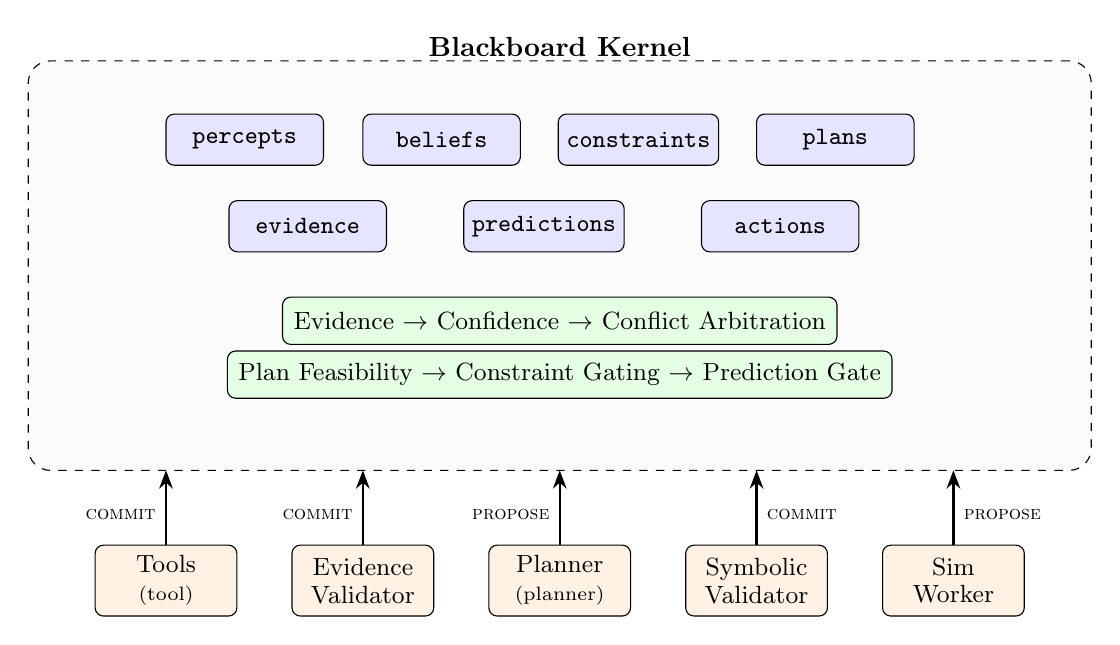
\begin{tikzpicture}[
  slot/.style={draw, rounded corners=3pt, minimum width=2.0cm, minimum height=0.65cm,
               font=\small\ttfamily, fill=blue!10, inner sep=3pt},
  role/.style={draw, rounded corners=3pt, minimum width=1.8cm, minimum height=0.9cm,
               font=\small, fill=orange!10, align=center, inner sep=3pt},
  pipenode/.style={draw, rounded corners=3pt, fill=green!10, font=\small,
                   minimum height=0.6cm, inner sep=4pt},
  node distance=0.4cm,
]
  % --- Kernel boundary ---
  \node[draw, dashed, rounded corners=8pt, fill=gray!3,
        minimum width=13.5cm, minimum height=5.2cm,
        label={[font=\bfseries, yshift=-2pt]above:Blackboard Kernel}]
        (kernel) at (0, 1.0) {};

  % --- Slot row 1 (top) ---
  \node[slot] (percepts)    at (-4,  2.6) {percepts};
  \node[slot] (beliefs)     at (-1.5, 2.6) {beliefs};
  \node[slot] (constraints) at ( 1,  2.6) {constraints};
  \node[slot] (plans)       at ( 3.5, 2.6) {plans};

  % --- Slot row 2 ---
  \node[slot] (evidence)    at (-3.2, 1.5) {evidence};
  \node[slot] (predictions) at (-0.2, 1.5) {predictions};
  \node[slot] (actions)     at ( 2.8, 1.5) {actions};

  % --- Validation pipeline (two lines, stacked) ---
  \node[pipenode] (val1) at (0, 0.3)
    {Evidence $\to$ Confidence $\to$ Conflict Arbitration};
  \node[pipenode, below=2pt of val1] (val2)
    {Plan Feasibility $\to$ Constraint Gating $\to$ Prediction Gate};

  % --- External roles (well below kernel boundary) ---
  % kernel bottom edge is at y = 1.0 - 2.6 = -1.6
  \node[role] (tools)   at (-5.0, -3.0) {Tools\\[-1pt]{\scriptsize(tool)}};
  \node[role] (evval)   at (-2.5, -3.0) {Evidence\\[-1pt]Validator};
  \node[role] (planner) at ( 0.0, -3.0) {Planner\\[-1pt]{\scriptsize(planner)}};
  \node[role] (symval)  at ( 2.5, -3.0) {Symbolic\\[-1pt]Validator};
  \node[role] (simw)    at ( 5.0, -3.0) {Sim\\[-1pt]Worker};

  % --- Arrows from roles to kernel boundary bottom ---
  \draw[-Stealth, thick] (tools.north) -- (-5.0, -1.6)
    node[left, font=\scriptsize, pos=0.4] {\textsc{commit}};
  \draw[-Stealth, thick] (evval.north) -- (-2.5, -1.6)
    node[left, font=\scriptsize, pos=0.4] {\textsc{commit}};
  \draw[-Stealth, thick] (planner.north) -- (0.0, -1.6)
    node[left, font=\scriptsize, pos=0.4] {\textsc{propose}};
  \draw[-Stealth, thick] (symval.north) -- (2.5, -1.6)
    node[right, font=\scriptsize, pos=0.4] {\textsc{commit}};
  \draw[-Stealth, thick] (simw.north) -- (5.0, -1.6)
    node[right, font=\scriptsize, pos=0.4] {\textsc{propose}};

\end{tikzpicture}
\caption{Architecture overview. Seven semantic slots on the shared blackboard, accessed through role-based permissions. Tools commit percepts; evidence validators commit evidence artifacts; the planner proposes beliefs, plans, actions, and predictions; symbolic validators commit constraints; the simulator worker proposes predictions (committed by the kernel after validation). The validation pipeline mediates all state transitions from \textsc{propose} to \textsc{commit}.}
\label{fig:architecture}
\end{figure}

\subsection{Typed State Slots}

The kernel organizes all internal state into seven semantic slots (Table~\ref{tab:slots}). Each slot has a designated write mode and commit authority, enforcing separation of concerns at the data level.

\begin{table}[ht]
\centering
\begin{tabular}{@{}llll@{}}
\toprule
\textbf{Slot} & \textbf{Description} & \textbf{Mode} & \textbf{Commit Auth.} \\
\midrule
percepts    & Raw observations           & commit                & tools \\
beliefs     & Interpreted state          & propose $\to$ commit  & kernel \\
constraints & Invariants / rules         & commit                & symbolic \\
plans       & Action sequences           & propose               & kernel (val.) \\
evidence    & Justification artifacts    & commit                & validators \\
predictions & Forward dynamics           & propose $\to$ commit  & kernel \\
actions     & External effects           & propose $\to$ commit  & kernel \\
\bottomrule
\end{tabular}
\caption{The 7 semantic slots with their write modes and commit authority.}
\label{tab:slots}
\end{table}

\subsection{Propose-Commit Semantics}

All mutable state follows a two-phase protocol:

\begin{enumerate}[nosep,leftmargin=1.5em]
  \item \textbf{Propose} --- Components may suggest updates.
  \item \textbf{Commit} --- Kernel commits only if: evidence is present and non-stale; no unresolved conflicts (or conflicts arbitrated by high-confidence source); source confidence exceeds minimum threshold; constraints are satisfied; plan feasibility confirmed.
\end{enumerate}

Narrative confidence is insufficient for commitment.

\subsection{Deterministic Execution Loop}

\begin{lstlisting}[language={}]
t0  Tools commit percepts (confidence, TTL)
t1  Planner reads percepts + beliefs
t2  Planner proposes belief updates
t3  Kernel validates evidence (stale, conflict, confidence)
t4  Kernel arbitrates conflicts via confidence thresholds
t5  Beliefs committed or rejected; evidence artifact recorded
t6  Planner proposes plan (sequence of intended actions)
t7  Kernel validates plan feasibility (beliefs + constraints)
t8  Planner proposes action from validated plan
t9  Kernel gates action via symbolic validation
t10 Action committed or halted; fallback queued
\end{lstlisting}

This loop is invariant across tasks and domains. Figure~\ref{fig:architecture} shows the architectural components; the execution flow follows the t0--t10 sequence above.


%% ============================================================
\section{Baseline Failure Walkthroughs}

\subsection{Scenario: Action with Stale Evidence}

\paragraph{String-Glue Agent.}
Tool returns stale data $\to$ planner infers action warranted $\to$ action executed immediately $\to$ error discovered later.
\textbf{Failure:} unsupported belief and unsafe action.

\paragraph{BK Agent (Same Inputs).}
Tool commits percept with \texttt{stale=true} $\to$ planner proposes belief $\to$ kernel rejects (stale evidence) $\to$ plan validation fails (missing belief) $\to$ action blocked $\to$ escalation queued.
\textbf{Outcome:} no incorrect action executed.

\subsection{Scenario: Action with Conflicting Evidence}

\paragraph{String-Glue Agent.}
Tool returns conflicting data $\to$ planner ignores conflict flag $\to$ action executed.
\textbf{Failure:} action based on unresolved conflict.

\paragraph{BK Agent (Same Inputs).}
Tool commits percept with \texttt{conflict=true}, confidence=0.3 $\to$ kernel detects conflict, attempts arbitration $\to$ confidence (0.3) below threshold (0.7) $\to$ belief rejected (\texttt{UNRESOLVED\_CONFLICT}) $\to$ escalation queued.
\textbf{Outcome:} conflict surfaced, not suppressed.


%% ============================================================
\section{Formal Architecture Specification}

\subsection{Record Structure}

\begin{lstlisting}[language={}]
record:
  id: "{slot}:{trace_id}:{n}"
  slot: beliefs | percepts | constraints |
        plans | evidence | predictions | actions
  mode: propose | commit
  kind: <domain-defined identifier>
  payload: <arbitrary structured data>
  provenance:
    writer_id: <role>
    trace_id: <correlation identifier>
    ts_ms: <millisecond timestamp>
    input_refs: [<record ids>]
    confidence: <float, optional>
    ttl_ms: <int, optional>
  evidence_refs: [<evidence record ids>]
  status: ACTIVE | INVALIDATED | EXPIRED
  scope: episode | persistent
\end{lstlisting}

Belief commitment requires valid \texttt{evidence\_refs}. Invalidated proposals carry a machine-readable \texttt{reason} (e.g., \texttt{STALE\_EVIDENCE}, \texttt{UNRESOLVED\_CONFLICT}, \texttt{LOW\_CONFIDENCE}). Records with \texttt{scope: persistent} survive across episodes within a shared kernel instance.

\subsection{Constraint Enforcement}

Constraints are declarative and domain-agnostic~\cite{leveson2011engineering,garcez2019neural}:

\begin{lstlisting}[language={}]
{
  "name": "no_duplicate_refund",
  "enabled": true,
  "blocks_field": "is_duplicate"
}
\end{lstlisting}

Actions declare required beliefs:

\begin{lstlisting}[language={}]
{
  "type": "issue_refund",
  "requires_beliefs": ["refund_due"],
  "is_duplicate": false
}
\end{lstlisting}

The kernel checks both declaratively---no domain-specific logic in the validation pipeline. The same mechanism generalizes to any domain: a monitoring system might define \texttt{block\_stale\_actions} using the identical constraint engine.


%% ============================================================
\section{Experimental Setup}

\subsection{Systems Compared}

We compare four agent architectures of increasing sophistication (Table~\ref{tab:systems}). The first three use deterministic planners; the fourth replaces the planner with a live language model while keeping the identical kernel validation pipeline.

\begin{table}[ht]
\centering
\begin{tabular}{@{}lll@{}}
\toprule
\textbf{System} & \textbf{Orchestration} & \textbf{Planner} \\
\midrule
String Glue & Free-form text pipeline      & Deterministic \\
JSON Glue   & Structured + confidence      & Deterministic \\
BK          & Governed blackboard kernel   & Deterministic \\
LLM+BK     & Governed blackboard kernel   & GPT-OSS-20B / Qwen3-80B \\
\bottomrule
\end{tabular}
\caption{Systems compared. The first three are deterministic; the LLM+BK agent uses live language models served via OpenAI-compatible APIs. The kernel validation pipeline is identical across all BK variants.}
\label{tab:systems}
\end{table}

\subsection{Tasks}

\textbf{Benchmark domain: Stripe payment refunds.} Six tasks covering distinct failure modes:

\begin{itemize}[nosep,leftmargin=1.5em]
  \item \texttt{stripe\_refund\_clean} --- Clean charge data (happy path)
  \item \texttt{stripe\_refund\_stale} --- Stale charge records
  \item \texttt{stripe\_refund\_conflict} --- Conflicting payment data
  \item \texttt{stripe\_refund\_duplicate} --- Duplicate refund blocking
  \item \texttt{stripe\_refund\_tool\_failure} --- API failure / missing data
  \item \texttt{stripe\_refund\_combined} --- Combined perturbation factors
\end{itemize}

50 seeded runs per task per agent = 1,200 total episodes. Perturbation rates (deterministic, seed-based): stale data (10\%), conflicting sources (10\%), low-confidence evidence (10\%), partial tool failure (5\%).

The kernel contains zero domain-specific logic. Domain agnosticity is further demonstrated through a separate multi-episode monitoring system (\texttt{examples/multi\_episode.py}) that uses the identical kernel with temperature sensors, anomaly detection, and adaptive constraint learning.

\subsection{Metrics}

\begin{itemize}[nosep,leftmargin=1.5em]
  \item \textbf{Task success} --- correct decision given evidence state and constraints
  \item \textbf{Unsafe action commits} --- action executed when evidence was tainted or constraint violated
  \item \textbf{Unsupported beliefs} --- belief held without valid evidence
  \item \textbf{Traceability} --- decision chain from action to evidence fully inspectable
  \item \textbf{Failure transparency} --- failures surfaced as explicit codes vs.\ silent errors
\end{itemize}


%% ============================================================
\section{Results}

\subsection{Aggregate Outcomes (1,200 episodes)}

Table~\ref{tab:results} summarizes performance across all five metrics.

\begin{table}[H]
\centering
\begin{tabular}{@{}lcccc@{}}
\toprule
\textbf{Metric} & \textbf{String Glue} & \textbf{JSON Glue} & \textbf{BK} & \textbf{LLM+BK} \\
\midrule
Task success         & 0.613 & 0.570 & 1.000 & 0.990 \\
Unsafe actions       & 0.387 & 0.430 & 0.000 & 0.000 \\
Unsupported beliefs  & 0.260 & 0.310 & 0.000 & 0.000 \\
Traceability         & 0.100 & 0.300 & 1.000 & 1.000 \\
Failure transparency & 0.100 & 0.300 & 1.000 & 1.000 \\
\bottomrule
\end{tabular}
\caption{Aggregate results across 1,200 episodes (6 Stripe refund tasks, 50 seeds, 4 agents). Both BK variants achieve zero unsafe actions.}
\label{tab:results}
\end{table}

Both BK variants achieve zero unsafe actions across all 1,200 episodes, regardless of whether the planner is deterministic or LLM-based. The deterministic BK agent achieves perfect task success (1.000); the LLM+BK agent achieves 0.990, with 3 failures out of 300 episodes (all on \texttt{stripe\_refund\_tool\_failure}). Baseline agents produce unsafe actions in 38.7--43.0\% of episodes. JSON Glue performs worse than String Glue on task success (0.570 vs 0.613) because it computes confidence scores that reflect data quality but never acts on them---metadata without governance is cosmetic.

%% --- Figure 2: Results Visualization ---
\begin{figure}[ht]
\centering
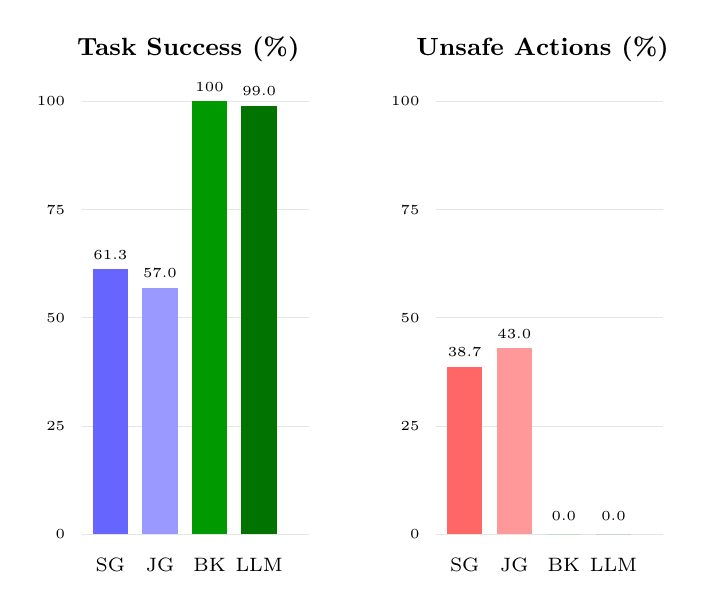
\begin{tikzpicture}[
  yscale=0.055, xscale=0.9,
]
  % --- Task Success ---
  \node[font=\small\bfseries] at (1.5, 112) {Task Success (\%)};
  \draw[gray!40] (0,0) -- (3.2,0);
  \foreach \y in {0,25,50,75,100} {
    \draw[gray!20] (0,\y) -- (3.2,\y);
    \node[font=\tiny, anchor=east] at (-0.1,\y) {\y};
  }

  \fill[blue!60] (0.15,0) rectangle (0.65,61.3);
  \fill[blue!40] (0.85,0) rectangle (1.35,57.0);
  \fill[green!60!black] (1.55,0) rectangle (2.05,100);
  \fill[green!45!black] (2.25,0) rectangle (2.75,99.0);

  \node[font=\scriptsize] at (0.4,-7) {SG};
  \node[font=\scriptsize] at (1.1,-7) {JG};
  \node[font=\scriptsize] at (1.8,-7) {BK};
  \node[font=\scriptsize] at (2.5,-7) {LLM};

  \node[font=\tiny, above] at (0.4,61.3) {61.3};
  \node[font=\tiny, above] at (1.1,57.0) {57.0};
  \node[font=\tiny, above] at (1.8,100) {100};
  \node[font=\tiny, above] at (2.5,99.0) {99.0};

  % --- Unsafe Actions ---
  \begin{scope}[xshift=5cm]
  \node[font=\small\bfseries] at (1.5, 112) {Unsafe Actions (\%)};
  \draw[gray!40] (0,0) -- (3.2,0);
  \foreach \y in {0,25,50,75,100} {
    \draw[gray!20] (0,\y) -- (3.2,\y);
    \node[font=\tiny, anchor=east] at (-0.1,\y) {\y};
  }

  \fill[red!60] (0.15,0) rectangle (0.65,38.7);
  \fill[red!40] (0.85,0) rectangle (1.35,43.0);
  \fill[green!60!black] (1.55,0) rectangle (2.05,0);
  \fill[green!45!black] (2.25,0) rectangle (2.75,0);

  \node[font=\scriptsize] at (0.4,-7) {SG};
  \node[font=\scriptsize] at (1.1,-7) {JG};
  \node[font=\scriptsize] at (1.8,-7) {BK};
  \node[font=\scriptsize] at (2.5,-7) {LLM};

  \node[font=\tiny, above] at (0.4,38.7) {38.7};
  \node[font=\tiny, above] at (1.1,43.0) {43.0};
  \node[font=\tiny, above] at (1.8,1) {0.0};
  \node[font=\tiny, above] at (2.5,1) {0.0};
  \end{scope}
\end{tikzpicture}
\caption{Task success and unsafe actions across 1,200 episodes. SG = String Glue, JG = JSON Glue, BK = deterministic kernel, LLM = LLM+BK. BK agents (green) achieve near-perfect success with zero unsafe actions; baseline agents (blue/red) produce unsafe actions in 38.7--43.0\% of episodes.}
\label{fig:results}
\end{figure}

\subsection{Per-Task Breakdown (BK Agents)}

\begin{table}[ht]
\centering
\begin{tabular}{@{}lccc@{}}
\toprule
\textbf{Task} & \textbf{BK Success} & \textbf{LLM+BK Success} & \textbf{LLM+BK Unsafe} \\
\midrule
clean          & 1.000 & 1.000 & 0.000 \\
stale          & 1.000 & 1.000 & 0.000 \\
conflict       & 1.000 & 1.000 & 0.000 \\
duplicate      & 1.000 & 1.000 & 0.000 \\
tool\_failure  & 1.000 & 0.940 & 0.000 \\
combined       & 1.000 & 1.000 & 0.000 \\
\bottomrule
\end{tabular}
\caption{Per-task results for BK agents. Task names are prefixed with \texttt{stripe\_refund\_}.}
\label{tab:pertask}
\end{table}

The \texttt{tool\_failure} task (0.940 success for LLM+BK) is the one scenario where the LLM occasionally declines to propose---3 out of 50 episodes. The deterministic BK achieves 1.000 on the same task, confirming this is a planner limitation, not a governance limitation. The LLM never produces an unsafe action on any task.

\subsection{Domain Agnosticity}

To validate that governance generalizes beyond Stripe, the kernel is demonstrated in a separate domain: a temperature monitoring system with five workers (sensor, analyst, simulator, actuator, adaptive) running across $N$ episodes. The kernel code is identical---only workers, tools, and domain semantics change. See Section~\ref{sec:multiepisode} for details.


\subsection{Representative BK Trace (Stale Evidence)}

\begin{lstlisting}[language={}]
t0  percept.charge committed (stale=true)
t2  belief.refund_due proposed
t3  evidence validation: STALE_EVIDENCE -- belief rejected
t5  plan.action_plan proposed
t6  plan validation: PLAN_MISSING_BELIEF -- plan rejected
t8  action.queue_for_review proposed
t9  action.queue_for_review committed
\end{lstlisting}

The kernel detects stale evidence at t3 and rejects the belief. Without a committed belief, the plan fails feasibility. The agent falls back to \texttt{queue\_for\_review}---a safe action that does not execute the refund.

\subsection{Representative BK Trace (Conflict Arbitration)}

\begin{lstlisting}[language={}]
t0  percept.charge committed (conflict=true, confidence=0.8)
t2  belief.refund_due proposed
t3  evidence validation: CONFLICTING_EVIDENCE detected
t4  arbitration: confidence 0.8 >= threshold 0.7 -- resolved
t5  evidence artifact recorded
t6  belief.refund_due committed
t7  plan.action_plan proposed -- feasible
t8  action.issue_refund proposed
t9  action.issue_refund committed
\end{lstlisting}

Conflict resolution is deterministic and auditable---the confidence threshold, not the planner, decides.

\subsection{LLM Planner Integration}

To validate that BK governance holds with a non-deterministic planner, we replaced the deterministic planner with live language models (GPT-OSS-20B, Qwen3-80B) served via OpenAI-compatible APIs. The kernel validation pipeline remains identical.

\paragraph{Governed Schema.}
The LLM decides \emph{whether} to propose, but the agent governs the schema: belief names and dependencies are fixed by the agent (\texttt{refund\_due}, \texttt{depends\_on: ["charge"]}), not the LLM. Plan steps always declare \texttt{requires\_beliefs} referencing the task's belief. Action payloads use the agent's refund fields, not LLM-generated values.

\paragraph{Prompt Bypass Attempts.}
During development, an initial untuned LLM planner exhibited two failure modes: (1)~over-caution (declining to propose in the majority of episodes) and (2)~governance bypass (proposing plans with empty \texttt{requires\_beliefs}, circumventing the belief-dependency check). The kernel caught both: over-caution resulted in safe fallback actions, while bypass attempts were rejected by the validation pipeline. Both failure modes were subsequently eliminated through prompt tuning and governed schema. After tuning, the LLM+BK agent achieved 0.990 task success and 0.000 unsafe actions across 300 episodes.

\paragraph{Implication.}
The v1 results demonstrate that an ungoverned LLM planner \emph{will} find ways to circumvent safety. The kernel catches both failure modes. Governance is the mechanism; the LLM is a replaceable component within it.


%% ============================================================
\section{From Governance Layer to Cognitive Substrate}

The benchmark results demonstrate that governance solves the orchestration problem. But governance alone addresses \emph{outputs} of reasoning---it doesn't provide infrastructure for \emph{better} reasoning. Current LLMs lack persistent state, world models, and learning from experience. We extend the kernel into a \textbf{general cognitive substrate} with six capabilities, drawing on ideas from cognitive science~\cite{baars1988cognitive,dehaene2017consciousness} and predictive world models~\cite{lecun2022path,ha2018world,hafner2020dream}.

\subsection{Worker Protocol and Orchestrator}

Rather than hardcoding agent pipelines, we define a \texttt{Worker} protocol with fields: \texttt{worker\_id}, \texttt{role}, \texttt{reads}, \texttt{writes}, \texttt{should\_activate()}, and \texttt{step()}. Any component satisfying this protocol can be registered with the \texttt{Orchestrator}, which runs workers in dependency order until quiescence or a round limit. Worker exceptions are caught per-worker; a failing worker does not halt the loop.

\subsection{Session-Scoped Persistence and Adaptive Learning}

Records gain a \texttt{scope} field: \texttt{"episode"} (default) or \texttt{"persistent"}. The \texttt{AdaptiveWorker} implements outcome-driven constraint learning: between episodes, it scans the store for invalidated records and commits persistent constraints when a failure pattern exceeds a threshold.

In a 20-episode demonstration (seed=7): after 2 stale-evidence rejections, it derived \texttt{block\_stale\_actions} at episode 4; after 2 negative-prediction rejections, it derived \texttt{block\_negative\_predictions} at episode 12. Neither constraint was scripted.

\subsection{Prediction Slot and Simulator Worker}

A seventh slot, \texttt{predictions}, provides governed forward dynamics. The \texttt{SimulatorWorker} fills this slot using declarative \texttt{SimRule} definitions with condition operators (\texttt{gt}, \texttt{lt}, \texttt{gte}, \texttt{lte}, \texttt{ne}, \texttt{eq}). Actions can optionally require a committed prediction with non-negative expected outcome.

\subsection{Pluggable Store with SQLite Implementation}

The \texttt{StoreProtocol} extracts the store interface into an explicit contract (6 methods: \texttt{append}, \texttt{get}, \texttt{list\_slot}, \texttt{find\_active\_by\_kind}, \texttt{invalidate}, \texttt{close}). \texttt{SqliteStore} provides production persistence with WAL journaling and indexed queries.

\subsection{What the Substrate Addresses}

\begin{table}[ht]
\centering
\begin{tabular}{@{}p{3.5cm}p{4cm}p{4.5cm}@{}}
\toprule
\textbf{LLM Limitation} & \textbf{Mechanism} & \textbf{Implementation} \\
\midrule
No persistent state & Session-scoped records & SqliteStore + Session \\
No world model & Prediction slot + sim workers & SimulatorWorker + SimRule \\
Hallucination & Propose/commit + evidence val. & EvidenceValidator \\
Can't self-constrain & Constraint gating & SymbolicValidator \\
No learning & Adaptive workers & AdaptiveWorker \\
Monolithic reasoning & Worker protocol & Orchestrator \\
\bottomrule
\end{tabular}
\caption{How the cognitive substrate addresses fundamental LLM limitations.}
\label{tab:substrate}
\end{table}

\subsection{Multi-Episode Demonstration}
\label{sec:multiepisode}

The substrate is demonstrated in \texttt{examples/multi\_episode.py}: a domain-agnostic monitoring system with five workers running across $N$ episodes.

\begin{lstlisting}[language={}]
Ep  0 | temp= 87.0 stale=True  | belief=N pred=-     | NO_ACTION
Ep  2 | temp=108.0              | belief=Y pred=1.0   | ALERT
Ep  3 | temp= 86.0 stale=True  | belief=N pred=-     | NO_ACTION
  >> LEARNED: ['block_stale_actions']
Ep  5 | temp= 81.0              | belief=Y pred=-0.5  | REVIEW
  >> LEARNED: ['block_negative_predictions']
Ep 12 | temp= 93.0              | belief=Y pred=1.0   | ALERT
\end{lstlisting}

Both constraints persist via \texttt{scope="persistent"} and were derived from observed failure patterns---not scripted.


%% ============================================================
\section{Limitations and Misuse Risks}

BK does not replace human oversight and cannot correct flawed constraint definitions. The controlled evaluation uses a single domain (Stripe payment refunds) with 1,200 episodes. While a separate multi-episode monitoring demonstration confirms that the kernel generalizes to other domains with unchanged code, formal multi-domain evaluation at the same scale remains future work. LLM planner integration has been validated with GPT-OSS-20B and Qwen3-80B; additional model diversity (different architectures, parameter scales) would strengthen generalization claims. Generalization to multi-turn dialogues, adversarial prompt injection, and open-ended planning domains also remains future work.

The cognitive substrate extensions are production-implemented but carry their own limitations. The \texttt{SimulatorWorker} provides rule-based forward dynamics, not learned world models~\cite{ha2018world,hafner2020dream}. The \texttt{AdaptiveWorker} learns from failure-pattern frequency---a useful heuristic, but not causal inference. The \texttt{SqliteStore} is single-process; distributed deployments require a networked store. Misuse risks include constraint suppression and governance bypass, which require organizational controls beyond technical enforcement.


%% ============================================================
\section{Conclusion}

This study demonstrates that reliability in modular AI systems is limited not by model intelligence, but by architectural governance. By synthesizing established techniques---blackboard architectures~\cite{erman1980hearsay}, propose-commit protocols, evidence-gated validation, and role-based privilege separation---into a governance layer for agent orchestration, we eliminate an entire class of orchestration failures that persist across prompt tuning, schema enforcement, and reflection-based approaches~\cite{wang2023selfrefine}.

In a controlled evaluation of 1,200 episodes across 6 Stripe payment refund tasks, the deterministic BK agent achieves perfect task success (1.000) with zero unsafe actions, while the LLM-backed BK agent (GPT-OSS-20B / Qwen3-80B) achieves 0.990 task success with zero unsafe actions. Baseline agents produce unsafe actions in 38.7--43.0\% of episodes. The ungoverned LLM planner exhibited both over-caution and governance bypass---failure modes the kernel caught without model-specific or domain-specific logic.

Domain agnosticity is demonstrated architecturally: the kernel contains zero domain-specific logic, and a separate multi-episode monitoring system uses the identical kernel with temperature sensors, anomaly detection, and adaptive constraint learning.

The evolution from governance layer to cognitive substrate extends this foundation to address fundamental LLM limitations through production implementations: \texttt{SqliteStore} for persistence, \texttt{SimulatorWorker} for forward dynamics, \texttt{AdaptiveWorker} for constraint learning, and \texttt{Orchestrator} for composable worker execution. The substrate retains full backward compatibility while demonstrating genuine adaptive behavior: in a 20-episode run, the system independently derived two persistent constraints from failure-pattern analysis.

As AI systems become more autonomous, governed cognition emerges as a foundational requirement for trustworthy deployment.


%% ============================================================
\bibliographystyle{plain}
\bibliography{references}

\end{document}
